% !TEX root = ../thesis-example.tex
%
\chapter{Multiple time series forecasting using quasi-randomized functional link neural networks}
\label{sec:rvfl_mts}

\section{Introduction}

In this paper, we are interested in obtaining forecasts for multiple time series, by taking into account the potential nonlinear relationships between their observations. This type of problem has been tackled recently by \cite{exterkate2016nonlinear}, who applied kernel regularized least squares to a set of macroeconomic time series. The Long Short-Term Memory neural networks (LSTM) architectures (introduced by \cite{hochreiter1997long}) are another family of models, which are currently widely used for this purpose. As a basis for our model, we will use (quasi-)randomized neural networks known as Random Vector Functional Link neural networks (RVFL networks hereafter)

\medskip

The forecasting method described in this paper, provides useful inputs for Insurance quantitative Risk Management models; the interested reader can refer to \cite{bonnin2015retraite} for example.

\medskip

To the best of our knowledge, randomized neural networks were introduced by \cite{schmidt1992feedforward}, and the RVFL networks were introduced by \cite{pao1994learning}. An early approach for multivariate time series forecasting using neural networks is described in \cite{chakraborty1992forecasting}. They applied a \textit{back propagation} algorithm from \cite{rumelhart1988learning} to trivariate time series, and found that the combined training of the series gave better forecasts than a separate training of each individual series. The novelty of the approach described in this paper is to derive an RVFL model for multiple time series, under two separate regularization constraints on the parameters, as it will be described in details in  section ~\ref{solve_rvfl}.

\medskip

RVFL networks are \textit{multilayer feedforward} neural networks, in which there is a \textit{direct link} between the predictors and the output variable, aiming at capturing the linear relationships. In addition to the \textit{direct link}, there are new features: the hidden nodes (the dataset is augmented), that help to capture the nonlinear relationships between the time series. These new features are obtained by random simulation over a given interval. More details on the \textit{direct link} and the hidden nodes will be provided in the next section.

\medskip

The RVFL networks have been successfully applied to solving different types of classification and regression problems; see for example \cite{dehuri2010comprehensive}. More specifically, they have been applied to univariate time series forecasting by \cite{ren2016random}. A comprehensive survey can be found in \cite{zhang2016comprehensive}; where a large number of model specifications are tested on classification problems, including changing the range of hidden layer's randomization.

\medskip

Here, we will use RVFL networks with one hidden layer. And instead of relying on fully randomized nodes, we will use sequences of deterministic quasi-random numbers. Indeed, with fully randomized nodes, the model fits obtained are dependent on the choice of a simulation \textit{seed}. Typically, a different fitting solution would be obtained for each \textit{seed}.

\medskip

In our various numerical examples from section \ref{sec:numericalexamples}, we will apply the RVFL networks to forecasting trivariate time series, notably (but not only) in a Dynamic Nelson Siegel (DNS) framework (see \cite{nelson1987parsimonious}, \cite{diebold2006forecasting}). We will obtain point forecasts and predictive distributions  for the series, and see that in this RVFL framework, one (or more) variable(s) can be stressed, and influence the others. More precisely, about this last point, it means that it is possible, as in dynamic regression models (\cite{pankratz2012forecasting}) to assign a specific future value to one regressor, and obtain forecasts of the remaining variables. Another advantage of the model described here, is its ability to integrate multiple other exogenous variables, without overfitting in-sample data.

\section{Description of the model}

The general procedure for obtaining the model's optimal parameters and predictions is  summarized in figure \ref{fig:flowchart}. 

\begin{figure}[!htb]
\centering
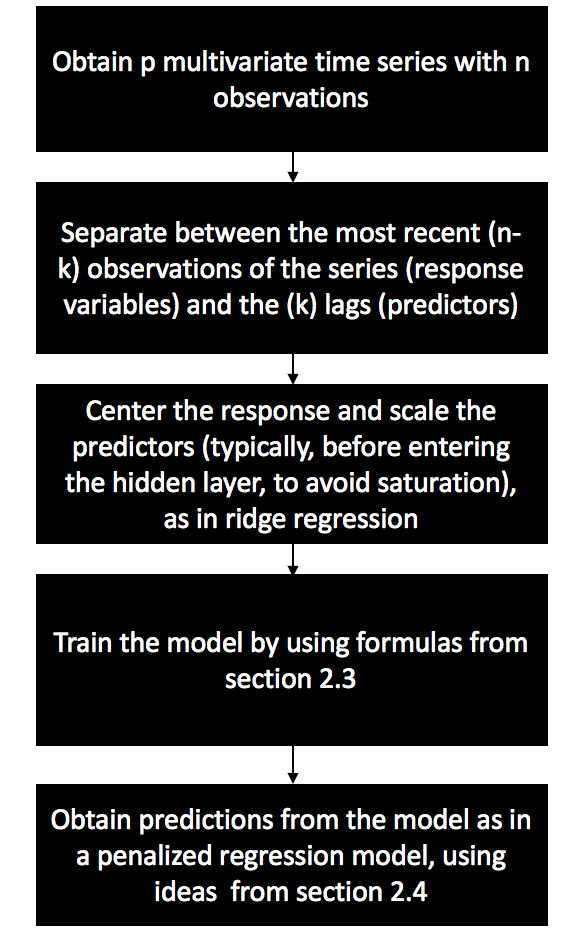
\includegraphics[width=5.5cm]{gfx/chapter-rvfl-mts/flowchart}
\caption{}
\label{fig:flowchart}
\end{figure}


This procedure is described in details in the next sections, especially sections \ref{solve_rvfl} and \ref{sec:preds}. 
